\appendix

\chapter{Charte \excilys{}}
\label{ann:charte}
\includepdf{annexes/charte_excilys.pdf}

\chapter{Test de charge de MF Banking}
\label{ann:gatling}
\begin{figure}[h!]
	\centering
		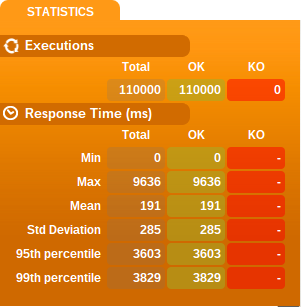
\includegraphics[scale=0.5]{images/global.pdf}
	\caption{Stastiques globales du test : nombre de requêtes réussies et échouées et détails du temps de réponse}
\end{figure}

\begin{figure}[h!]
	\centering
		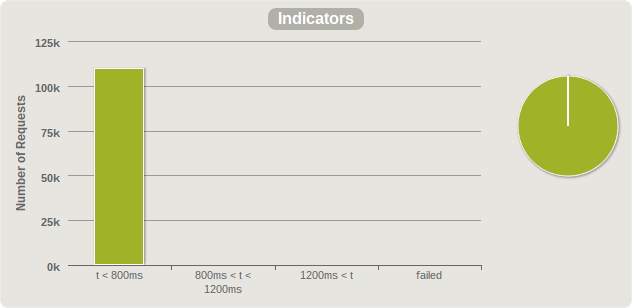
\includegraphics[scale=0.5]{images/indicators.pdf}
	\caption{On peut voir que presque toutes les requêtes ont été effectués en moins de 800 ms}
\end{figure}

\begin{figure}[h!]
	\centering
		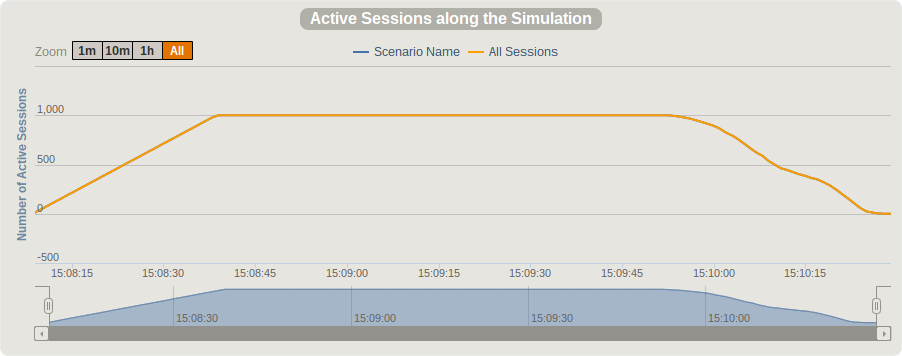
\includegraphics[scale=0.5]{images/active-sessions.pdf}
	\caption{Nombres d'utilisateurs actifs simultanément. La montée progressive du nombres d'utilisateurs au début est dû à une \textit{rampe} : on demande à Gatling de prendre 30 secondes pour lancer progressivement les 1000 utilisateurs du test}
\end{figure}

\begin{figure}[h!]
	\centering
		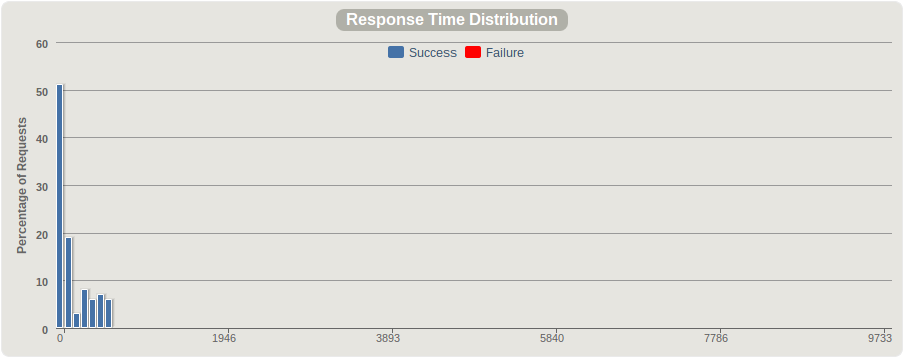
\includegraphics[scale=0.5]{images/response-time.pdf}
	\caption{Distribution du temps de réponse : on peut voir que la majorité des requêtes ont été été effectués quasi instantanément et que le nombre de requêtes lentes est tellement faible qu'elles n'apparaissent même pas sur le graphe}
\end{figure}

\begin{figure}[h!]
	\centering
		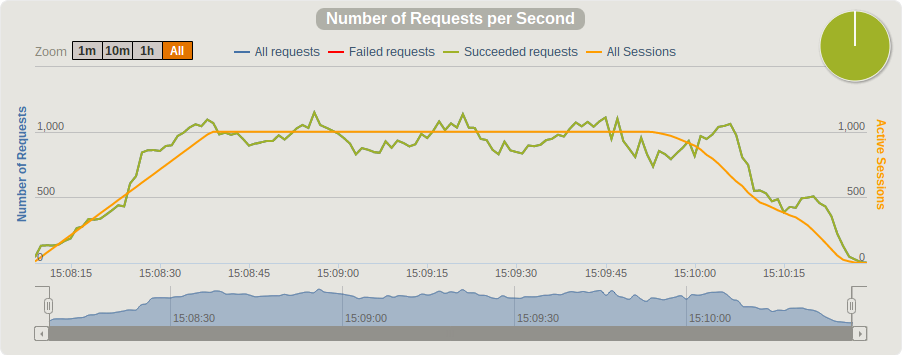
\includegraphics[scale=0.5]{images/requests.pdf}
	\caption{Nombre de requêtes qui démarrent par seconde : on observe qu'une fois la rampe terminée, le système se maintient sans difficulté entre 800 et 1200 requêtes par seconde}
\end{figure}

\begin{figure}[h!]
	\centering
		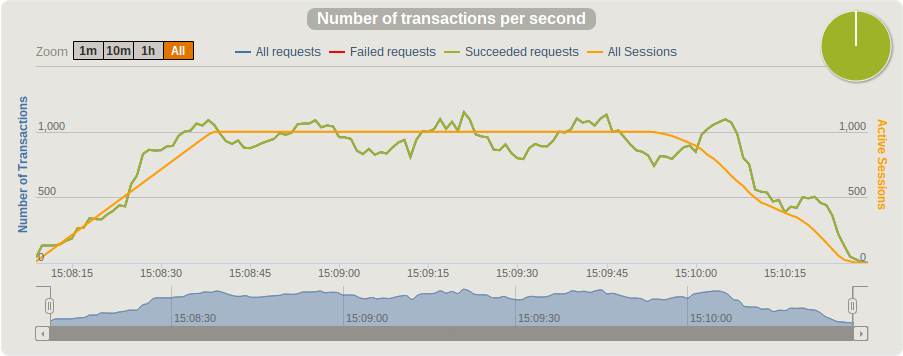
\includegraphics[scale=0.5]{images/transactions.pdf}
	\caption{Nombre de transactions (requêtes qui s'achèvent) par seconde : mêmes observations que pour les requêtes, le système se maintient durant tout le test entre 800 et 1200 transactions par seconde}
\end{figure}